
% Copyright (c) 2015 - 2020 Mario Mlačak, mmlacak@gmail.com
% Licensed and published as Public Domain work.

% Tamoanchan Revisited chapter ========================================
\chapter*{Tamoanchan Revisited}
\addcontentsline{toc}{chapter}{Tamoanchan Revisited}
\label{ch:Tamoanchan Revisited}

\begin{flushright}
\parbox{0.6\textwidth}{
\emph{I dream, therefore I exist. \\
\hspace*{\fill}{\textperiodcentered \textperiodcentered \textperiodcentered \hspace*{0.2em} August Strindberg} } }
\end{flushright}

\noindent
Tamoanchan Revisited is chess variant which is played on 22 x 22 board,
with white and bright cyan fields and light grey and grey pieces.
Star colors are yellow and bright red. In algebraic notation, columns
are enumerated from 'a' to 'v', and rows are enumerated from '1' to '22'.
A new piece is introduced, Serpent.

\clearpage % ..........................................................
% Serpent *************************************************************

\section*{Serpent}
\addcontentsline{toc}{section}{Serpent}
\label{sec:Tamoanchan Revisited/Serpent}

\noindent
\begin{wrapfigure}[11]{l}{0.4\textwidth}
\centering
\includegraphics[width=0.4\textwidth, keepaspectratio=true]{pieces/15_serpent.png}
\caption{Serpent}
\label{fig:15_serpent}
\end{wrapfigure}
Serpent moves diagonaly one field at the time, after which it alternates
diagonal.

All step-fields are also capture-fields, Serpent would be able to activate
not just Wave, but also Pyramid on any of them.

Serpent has movement limit, which is calculated from a board size of a variant
being played. In this variant Serpent can move for up to 14 fields, inclusively.

As an alternative move, Serpent can move one field vertically or horizontally
if it's unoccupied, to change color of accessible fields, and even teleport
while using color-changing move. Serpent can also diplace any Pawn in its way,
both own or opponent's.

% \vspace*{0.05\textheight}
\noindent
\begin{wrapfigure}{l}{0.4\textwidth}
\centering
\includegraphics[width=0.4\textwidth, keepaspectratio=true]{pieces/star/16_tamoanchan_revisited.png}
\caption{Star}
\label{fig:star/16_tamoanchan_revisited}
\end{wrapfigure}
Serpent can also initiate sacrificing of own Pawn, after which it can capture
multiple opponent's Pawns in a single move.

In algebraic notation symbol for Serpent is 'S'.

Star colors in this variant are presented on the left.

\clearpage % ..........................................................
% Movement ------------------------------------------------------------

\subsection*{Movement}
\addcontentsline{toc}{subsection}{Movement}
\label{sec:Tamoanchan Revisited/Serpent/Movement}

\noindent
\begin{wrapfigure}[8]{l}{0.4\textwidth}
\centering
\includegraphics[width=0.363636363636\textwidth, keepaspectratio=true]{examples/16_tr/scn_tr_01_serpent_diagonals.png}
\caption{Diagonals}
\label{fig:scn_tr_01_serpent_diagonals}
\end{wrapfigure}
On its first step Serpent can choose among any of the 4 diagonal fields,
i.e. either A or B diagonal.

On all subsequent steps Serpent has to alternate between diagonals.
Choice between 2 fields on a diagonal is independent of any previous choice.

\vspace*{0.04\textheight}
\noindent
\begin{wrapfigure}[5]{l}{0.4\textwidth}
\centering
\includegraphics[width=0.363636363636\textwidth, keepaspectratio=true]{examples/16_tr/scn_tr_02_serpent_1.png}
\caption{Step 1}
\label{fig:scn_tr_02_serpent_1}
\end{wrapfigure}
Starting position is marked S.

First step was taken onto upper-right field on diagonal B.
Next step has to be onto either field on diagonal A.

\vspace*{0.125\textheight}
\noindent
\begin{wrapfigure}[9]{l}{0.4\textwidth} % 7
\centering
\includegraphics[width=0.363636363636\textwidth, keepaspectratio=true]{examples/16_tr/scn_tr_03_serpent_2.png}
\caption{Step 2}
\label{fig:scn_tr_03_serpent_2}
\end{wrapfigure}
Step taken by Serpent was onto upper-left field on A diagonal.

Next step has to be on diagonal B, chosen freely between the 2 fields,
regardless of choice made for the first step.

\clearpage % ..........................................................

\vspace*{-1.2\baselineskip}
\noindent
\begin{wrapfigure}[6]{l}{0.4\textwidth}
\centering
\includegraphics[width=0.363636363636\textwidth, keepaspectratio=true]{examples/16_tr/scn_tr_04_serpent_3.png}
\vspace*{-0.5\baselineskip}
\caption{Step 3}
\label{fig:scn_tr_04_serpent_3}
\end{wrapfigure}
Last step was on B diagonal, next step has to alternate again, onto A diagonal.

Field numbers counts steps to them, and also gathered momentum.

\vspace*{2.7\baselineskip}
\noindent
\begin{wrapfigure}[4]{l}{0.4\textwidth}
\centering
\includegraphics[width=0.363636363636\textwidth, keepaspectratio=true]{examples/16_tr/scn_tr_05_serpent_end.png}
\vspace*{-0.5\baselineskip}
\caption{End step}
\label{fig:scn_tr_05_serpent_end}
\end{wrapfigure}
Finished move with 8 steps performed.

In this variant, Serpent is limited to 14 steps.

\vspace*{4.7\baselineskip}
\noindent
\begin{wrapfigure}[9]{l}{0.4\textwidth}
\centering
\includegraphics[width=0.363636363636\textwidth, keepaspectratio=true]{examples/16_tr/scn_tr_06_serpent_loop_illegal.png}
\vspace*{-0.5\baselineskip}
\caption{Loops are illegal}
\label{fig:scn_tr_06_serpent_loop_illegal}
\end{wrapfigure}
In a single ply Serpent can visit each field in its path only once.
So, loops within a single ply are illegal.

Fields visited in a previous ply (or, in a previous move) are accessible
without any limitations. So, loops within a single move are legal, if they
are closed in a ply other than starting ply of that loop.

\clearpage % ..........................................................

\subsubsection*{Static move is illegal}
\addcontentsline{toc}{subsubsection}{Static move is illegal}
\label{sec:Tamoanchan Revisited/Serpent/Movement/Static move is illegal}

% \vspace*{-1.2\baselineskip}
\noindent
\begin{wrapfigure}[8]{l}{0.4\textwidth}
\centering
\includegraphics[width=0.363636363636\textwidth, keepaspectratio=true]{examples/16_tr/scn_tr_07_static_move_is_illegal.png}
% \vspace*{-0.5\baselineskip}
\caption{Static move}
\label{fig:scn_tr_07_static_move_is_illegal}
\end{wrapfigure}
Static move is one in which a piece ends in the same position as it was at the
beginning of that same move. The same as in
\hyperref[fig:scn_mv_43_static_move_is_illegal_init]{previous example}, it's
illegal for a single Serpent in a move, or one starting a cascade, to end its
movement on its starting position.

% \clearpage % ..........................................................

% \vspace*{0.4\baselineskip}
\vspace*{1.4\baselineskip}
\subsubsection*{Static piece is illegal}
\addcontentsline{toc}{subsubsection}{Static piece is illegal}
\label{sec:Tamoanchan Revisited/Serpent/Movement/Static piece is illegal}

% \vspace*{-1.2\baselineskip}
\noindent
\begin{wrapfigure}[9]{l}{0.4\textwidth}
\centering
\includegraphics[width=0.363636363636\textwidth, keepaspectratio=true]{examples/16_tr/scn_tr_08_static_piece_is_illegal.png}
% \vspace*{-0.5\baselineskip}
\caption{Static piece}
\label{fig:scn_tr_08_static_piece_is_illegal}
\end{wrapfigure}
Unlike
\hyperref[fig:scn_mv_45_static_piece_is_legal_init]{previous example}, Serpent
activated in a cascade cannot, in the same ply, end its movement on its starting
field.

Here, Serpent activated in a cascade cannot return to its originating field S,
and so it cannot reactivate Wave, and force it to move over to e.g. field W.

\clearpage % ..........................................................

\subsubsection*{Revisiting fields, loops}
\addcontentsline{toc}{subsubsection}{Revisiting fields, loops}
\label{sec:Tamoanchan Revisited/Serpent/Movement/Revisiting fields, loops}

\vspace*{-1.2\baselineskip}
\noindent
\begin{figure}[!h]
\includegraphics[width=1.0\textwidth, keepaspectratio=true]{examples/16_tr/scn_tr_09_serpent_loop_init.png}
\caption{Serpent's first ply}
\label{fig:scn_tr_09_serpent_loop_init}
\end{figure}

While Serpent cannot revisit fields, and make loops in a single ply, Serpent can
do it in a new ply; either in a new move, or in the same move, if it has been
reactivated.

Here, Queen is about to activate Serpent via Wave A, which will then continue
cascade to Wave B, Bishop, and Wave C; Serpent's steps are also enumerated.

\clearpage % ..........................................................

\vspace*{-2.1\baselineskip}
\noindent
\begin{figure}[!h]
\includegraphics[width=1.0\textwidth, keepaspectratio=true]{examples/16_tr/scn_tr_10_serpent_loop_step.png}
\caption{Reactivating Serpent}
\label{fig:scn_tr_10_serpent_loop_step}
\end{figure}

Here, first part of cascade has been played out; grey arrows show path travelled
over by piece they point to. Wave C is now "in-the-air", about to reactivate light
Serpent with remaining 13 momentum.

Note, light Queen cannot return to its starting field Q, even if reactivated with
enough momentum, since it's
\hyperref[fig:scn_mv_43_static_move_is_illegal_init]{the very first piece in a cascade}.

\clearpage % ..........................................................

\vspace*{-2.1\baselineskip}
\noindent
\begin{figure}[!h]
\includegraphics[width=1.0\textwidth, keepaspectratio=true]{examples/16_tr/scn_tr_11_serpent_loop_end.png}
\caption{Serpent's second ply}
\label{fig:scn_tr_11_serpent_loop_end}
\end{figure}

. . .

\TODO

reactivated Serpent --> different ply --> can return to its starting field

\clearpage % ..........................................................

\subsubsection*{Different paths, momentum}
\addcontentsline{toc}{subsubsection}{Different paths, momentum}
\label{sec:Tamoanchan Revisited/Serpent/Movement/Different paths, momentum}

\vspace*{-1.2\baselineskip}
\noindent
\begin{wrapfigure}[9]{l}{0.4\textwidth}
\centering
\includegraphics[width=0.363636363636\textwidth, keepaspectratio=true]{examples/16_tr/scn_tr_12_serpent_path_short.png}
\vspace*{-0.5\baselineskip}
\caption{The shortest path}
\label{fig:scn_tr_12_serpent_path_short}
\end{wrapfigure}
While loops are illegal within single ply, it's still possible to find
different paths to the same destination, some of those with different
lengths, resulting in different accumulated momentum.

Example on the left shows the shortest path possible to activate Pyramid,
with 4 momentum.

% \clearpage % ..........................................................

\vspace*{0.3\baselineskip}
\noindent
\begin{wrapfigure}[4]{l}{0.4\textwidth}
\centering
\includegraphics[width=0.363636363636\textwidth, keepaspectratio=true]{examples/16_tr/scn_tr_13_serpent_path_long.png}
\vspace*{-0.5\baselineskip}
\caption{Long path}
\label{fig:scn_tr_13_serpent_path_long}
\end{wrapfigure}
Example on the left in the same situation now shows longer path available,
activating Pyramid with 8 momentum.

% \clearpage % ..........................................................

\vspace*{5.3\baselineskip}
\noindent
\begin{wrapfigure}[7]{l}{0.4\textwidth}
\centering
\includegraphics[width=0.363636363636\textwidth, keepaspectratio=true]{examples/16_tr/scn_tr_14_serpent_path_longer.png}
\vspace*{-0.5\baselineskip}
\caption{Longer path}
\label{fig:scn_tr_14_serpent_path_longer}
\end{wrapfigure}
One of the longest paths available in the same situation is shown on the left,
with 12 momentum accumulated.

Again, Serpent in this variant is limited to maximum of 14 steps performed in a
single ply.

\clearpage % ..........................................................

\subsubsection*{Color-changing move}
\addcontentsline{toc}{subsubsection}{Color-changing move}
\label{sec:Tamoanchan Revisited/Serpent/Movement/Color-changing move}

\noindent
\begin{minipage}{\textwidth}
\begin{wrapfigure}[9]{l}{0.4\textwidth}
\centering
\includegraphics[width=0.363636363636\textwidth, keepaspectratio=true]{examples/16_tr/scn_tr_15_serpent_neighbors.png}
\caption{Color-changing move}
\label{fig:scn_tr_15_serpent_neighbors}
\end{wrapfigure}
Serpent's alternative move is a way to change color of accessible fields,
provided that destination field is empty.

\mbox{}\newline % Forcing new paragraph ...
Color-changing fields are all fields immediately neighboring starting
location, either horizontally or vertically, but not diagonaly.
\end{minipage}

\vspace*{2.9\baselineskip}
\noindent
\begin{minipage}{\textwidth}
\begin{wrapfigure}[3]{l}{0.4\textwidth}
\centering
\includegraphics[width=0.363636363636\textwidth, keepaspectratio=true]{examples/16_tr/scn_tr_16_cascade_serpent_neighbors.png}
\caption{Color-changing cascade}
\label{fig:scn_tr_16_cascade_serpent_neighbors}
\end{wrapfigure}
Serpent's color-changing move can also be at the end of a cascade,
if Serpent was activated.
\end{minipage}

\clearpage % ..........................................................

\subsubsection*{Displacements while moving}
\addcontentsline{toc}{subsubsection}{Displacements while moving}
\label{sec:Tamoanchan Revisited/Serpent/Movement/Displacements while moving}

\vspace*{-1.2\baselineskip}
\noindent
\begin{wrapfigure}[11]{l}{0.4\textwidth}
\centering
\includegraphics[width=0.363636363636\textwidth, keepaspectratio=true]{examples/16_tr/scn_tr_17_displacement_init.png}
\vspace*{-0.5\baselineskip}
\caption{Before displacement}
\label{fig:scn_tr_17_displacement_init}
\end{wrapfigure}
Serpent can displace a Pawn it encounters and, in the same ply, continue its movement.
Displacement does not use momentum, and can be performed even if Serpent has none. Pawns,
own or opponent's, can be displaced; all other pieces cannot be displaced. \newline
\indent
Displacement fields are the same as color-changing fields, and also has to be empty;
i.e. a Pawn

\vspace*{-0.8\baselineskip}
\noindent
\begin{wrapfigure}[11]{l}{0.4\textwidth}
\centering
\includegraphics[width=0.363636363636\textwidth, keepaspectratio=true]{examples/16_tr/scn_tr_18_displacement_step.png}
\vspace*{-0.5\baselineskip}
\caption{Displacement step}
\label{fig:scn_tr_18_displacement_step}
\end{wrapfigure}
can be displaced for one field to the left, right, up, or bottom from
its encountered position, if that displacing field is empty. This is so, regardless
how displaced Pawn moves otherwise. \newline
\indent
Here, dark Pawn (now "in the air") can be displaced onto any of 3 empty neighboring
fields; down-field is illegal for displacement, since it's not empty.

\vspace*{-0.8\baselineskip}
\noindent
\begin{wrapfigure}[11]{l}{0.4\textwidth}
\centering
\includegraphics[width=0.363636363636\textwidth, keepaspectratio=true]{examples/16_tr/scn_tr_19_displacement_end.png}
\vspace*{-0.5\baselineskip}
\caption{Displacement end}
\label{fig:scn_tr_19_displacement_end}
\end{wrapfigure}
\indent
There is no limit to number of displacements Serpent can do in a ply. If there is no
empty displacement field, Serpent must either capture, or activate, or stop before
encountered Pawn. \newline
\indent
Here, dark Pawn has been displaced onto up-field; arrows show complete Serpent's
path in a single ply, grey before displacement, green after it.

\clearpage % ..........................................................

\TODO

displacements --> 1-by-1, in order of appearence --> 1st to field blocks later


\clearpage % ..........................................................

\subsubsection*{Out-of-board steps}
\addcontentsline{toc}{subsubsection}{Out-of-board steps}
\label{sec:Tamoanchan Revisited/Serpent/Movement/Out-of-board steps}

\vspace*{-1.0\baselineskip}
\noindent
\begin{figure}[!h]
\includegraphics[width=1.0\textwidth, keepaspectratio=true]{examples/16_tr/scn_tr_20_serpent_out_of_board.png}
\caption{Serpent out-of-board steps}
\label{fig:scn_tr_20_serpent_out_of_board}
\end{figure}

Here, light grey fields are virtual fields extending existing chessboard.
For Serpent, it's illegal to step outside chessboard, and all subsequent
steps are also illegal. That means, Serpent cannot reach fields 1 through
4 with selected path, even though it would end movement on the chessboard.

\clearpage % ..........................................................

\subsubsection*{Teleporting Serpent}
\addcontentsline{toc}{subsubsection}{Teleporting Serpent}
\label{sec:Tamoanchan Revisited/Serpent/Movement/Teleporting Serpent}

\vspace*{-1.0\baselineskip}
\noindent
\begin{figure}[!h]
\includegraphics[width=1.0\textwidth, keepaspectratio=true]{examples/16_tr/scn_tr_21_teleport_serpent_1.png}
\caption{Teleporting Serpent}
\label{fig:scn_tr_21_teleport_serpent_1}
\end{figure}

Serpent teleports to any empty portal-field near Star in opposite color
(here, fields 1 -- 6), just like
\hyperref[fig:scn_n_02_teleport_init]{any other piece, except Wave}.
Serpent is bound to fields in one color, similar to Bishop. Teleporting
Serpent presents opportunity to change color of available fields (here,
portal-fields 2, 5), also
\hyperref[fig:scn_n_14_teleport_bishop]{similar to Bishop}.

\clearpage % ..........................................................

\vspace*{-1.0\baselineskip}
\noindent
\begin{figure}[!h]
\includegraphics[width=1.0\textwidth, keepaspectratio=true]{examples/16_tr/scn_tr_22_teleport_serpent_2.png}
\caption{Color-changing step}
\label{fig:scn_tr_22_teleport_serpent_2}
\end{figure}

Serpent can also teleport by performing color-changing step. This also
gives opportunity for Serpent to change color of accessible fields. Note,
color changing portal-fields (here, fields 1, 3, 4, 6) are switched
compared to previous example.

\clearpage % ..........................................................

\subsubsection*{Pawn-sacrifice move}
\addcontentsline{toc}{subsubsection}{Pawn-sacrifice move}
\label{sec:Tamoanchan Revisited/Serpent/Movement/Pawn-sacrifice move}

\vspace*{-1.3\baselineskip}
\noindent
\begin{figure}[!h]
\includegraphics[width=1.0\textwidth, keepaspectratio=true]{examples/16_tr/scn_tr_23_pawn_sacrifice_init.png}
\caption{Pawn-sacrifice start}
\label{fig:scn_tr_23_pawn_sacrifice_init}
\end{figure}

Pawn-sacrifice move is initiated by Serpent activating Pyramid, which then
captures field at which own Pawn is located. Pawn is then
\hyperref[sec:Terms/Oblation]{oblationed}, and Serpent gets Pawn-sacrifice
tag and, in the same move, starts a new ply as if starting a new move. Any
received momentum (if Serpent was activated) is lost. Any of pieces involved
can be on any side of chessboard, own or opponent's.

\clearpage % ..........................................................

\vspace*{-2.1\baselineskip}
\noindent
\begin{figure}[!h]
\includegraphics[width=1.0\textwidth, keepaspectratio=true]{examples/16_tr/scn_tr_24_pawn_sacrifice_end.png}
\caption{Pawn-sacrifice end}
\label{fig:scn_tr_24_pawn_sacrifice_end}
\end{figure}

In a new ply, Serpent can capture all opponent's Pawns in it's path, or move over
empty fields. Serpent can't capture any other opponent's piece (here, dark Bishop).
Pawn-sacrifice tag lasts until normal limit of Serpent's ply is reached (in this
variant, 8 fields inclusively), or by any action other then capturing Pawns and
traversing empty fields, e.g. teleporting, activating Wave, ... Momentum Serpent
accumulates is counted from field at which it got Pawn-sacrifice tag.

% ------------------------------------------------------------ Movement
\clearpage % ..........................................................
% Activating Wave -----------------------------------------------------

\subsection*{Activating Wave}
\addcontentsline{toc}{subsection}{Activating Wave}
\label{sec:Tamoanchan Revisited/Serpent/Activating Wave}

% \vspace*{-1.0\baselineskip}
\noindent
\begin{wrapfigure}[3]{l}{0.4\textwidth}
\centering
\includegraphics[width=0.363636363636\textwidth, keepaspectratio=true]{examples/16_tr/scn_tr_25_serpent_activating_wave.png}
\caption{Activating}
\label{fig:scn_tr_25_serpent_activating_wave}
\end{wrapfigure}
Serpent can activate Wave on its step-fields only, it cannot activate Wave
on \hyperref[fig:scn_tr_15_serpent_neighbors]{color-changing fields}.

\vspace*{7.0\baselineskip}
\noindent
\begin{wrapfigure}[2]{l}{0.4\textwidth}
\centering
\includegraphics[width=0.363636363636\textwidth, keepaspectratio=true]{examples/16_tr/scn_tr_26_serpent_activated_wave.png}
\caption{Activated}
\label{fig:scn_tr_26_serpent_activated_wave}
\end{wrapfigure}
Activated Wave can freely choose any diagonal field for its first step.

\vspace*{8.0\baselineskip}
\noindent
\begin{wrapfigure}[2]{l}{0.4\textwidth}
\centering
\includegraphics[width=0.363636363636\textwidth, keepaspectratio=true]{examples/16_tr/scn_tr_27_serpent_activated_wave_step_1.png}
\caption{First step}
\label{fig:scn_tr_27_serpent_activated_wave_step_1}
\end{wrapfigure}
After first step, Wave must choose next step from the other diagonal.

\clearpage % ..........................................................

\noindent
\begin{figure}[!h]
\includegraphics[width=1.0\textwidth, keepaspectratio=true]{examples/16_tr/scn_tr_28_serpent_activated_wave_ply.png}
\caption{Activated Wave ply}
\label{fig:scn_tr_28_serpent_activated_wave_ply}
\end{figure}

Once the two directions are chosen, they cannot be changed, even if on a
proper diagonal. For instance, upon reaching field 6, it's illegal for Wave
to change movement to the other direction on B diagonal.

Unlike Serpent, Wave is not limited by number of steps. So, Wave can repeat
alternating between 2 chosen directions to the end of the chessboard.

\clearpage % ..........................................................

\subsubsection*{Out-of-board steps}
\addcontentsline{toc}{subsubsection}{Out-of-board steps}
\label{sec:Tamoanchan Revisited/Serpent/Activating Wave/Out-of-board steps}

\vspace*{-1.0\baselineskip}
\noindent
\begin{figure}[!h]
\includegraphics[width=1.0\textwidth, keepaspectratio=true]{examples/16_tr/scn_tr_29_wave_out_of_board.png}
\caption{Wave out-of-board steps}
\label{fig:scn_tr_29_wave_out_of_board}
\end{figure}

Again, light grey fields are virtual fields extending existing chessboard.
Wave activated by Serpent can step outside of a board, as long as its ply
ends on a board. Here, all enumerated step-fields 1 through 8 are reachable
by Wave, even though it stepped outside of the board. It is illegal for any
piece, including Wave, to end its ply outside of a board.

\clearpage % ..........................................................

\subsection*{Teleporting Wave}
\addcontentsline{toc}{subsection}{Teleporting Wave}
\label{sec:Tamoanchan Revisited/Serpent/Teleporting Wave}

\vspace*{-1.0\baselineskip}
\noindent
\begin{figure}[!h]
\includegraphics[width=1.0\textwidth, keepaspectratio=true]{examples/16_tr/scn_tr_30_off_board_teleport_wave.png}
\caption{Teleporting off-board Wave}
\label{fig:scn_tr_30_off_board_teleport_wave}
\end{figure}

Wave activated by Serpent can reach a Star and start teleporting, even
though it stepped outside of a chessboard. After teleporting, Wave emerges
from the other Star in the same color, in the opposite corner of a board.
Here, Wave started teleporting at light Star in upper-right corner, and
so it will emerge from light Star in lower-left corner.

\clearpage % ..........................................................

\vspace*{-1.0\baselineskip}
\noindent
\begin{figure}[!h]
\includegraphics[width=1.0\textwidth, keepaspectratio=true]{examples/16_tr/scn_tr_31_teleported_wave_on_board.png}
\caption{Teleported Wave}
\label{fig:scn_tr_31_teleported_wave_on_board}
\end{figure}

Wave has to continue alternating between 2 initialy selected directions (here,
A and B), even across teleportation. Since Wave dived into a Star from B direction,
next step after teleporting has to be in A direction. Again, Wave cannot change
directions from those initially selected; e.g. upon reaching field 9, it cannot
choose the other direction on B diagonal.

\clearpage % ..........................................................

\vspace*{-1.0\baselineskip}
\noindent
\begin{figure}[!h]
\includegraphics[width=1.0\textwidth, keepaspectratio=true]{examples/16_tr/scn_tr_32_on_board_teleport_wave.png}
\caption{Teleporting Wave}
\label{fig:scn_tr_32_on_board_teleport_wave}
\end{figure}

Similar to previous example, Wave activated by Serpent starts teleporting at
light Star in upper-right corner of a board, by stepping in A direction.

\clearpage % ..........................................................

\vspace*{-1.0\baselineskip}
\noindent
\begin{figure}[!h]
\includegraphics[width=1.0\textwidth, keepaspectratio=true]{examples/16_tr/scn_tr_33_teleported_wave_off_board.png}
\caption{Wave teleported off-board}
\label{fig:scn_tr_33_teleported_wave_off_board}
\end{figure}

Wave emerges from light Star in lower-left corner, starting with step in B
direction. All enumerated fields (here, 1 to 10) are reachable by teleported
Wave, even though it stepped outside of a board. Note, field 3 is blocked by
dark Pyramid, but Wave can continue past it, and e.g. activate light Pawn.

% ----------------------------------------------------- Activating Wave
% ************************************************************* Serpent
\clearpage % ..........................................................

\section*{Rush, en passant}
\addcontentsline{toc}{section}{Rush, en passant}
\label{sec:Tamoanchan Revisited/Rush, en passant}

\vspace*{-1.2\baselineskip}
\noindent
\begin{figure}[!h]
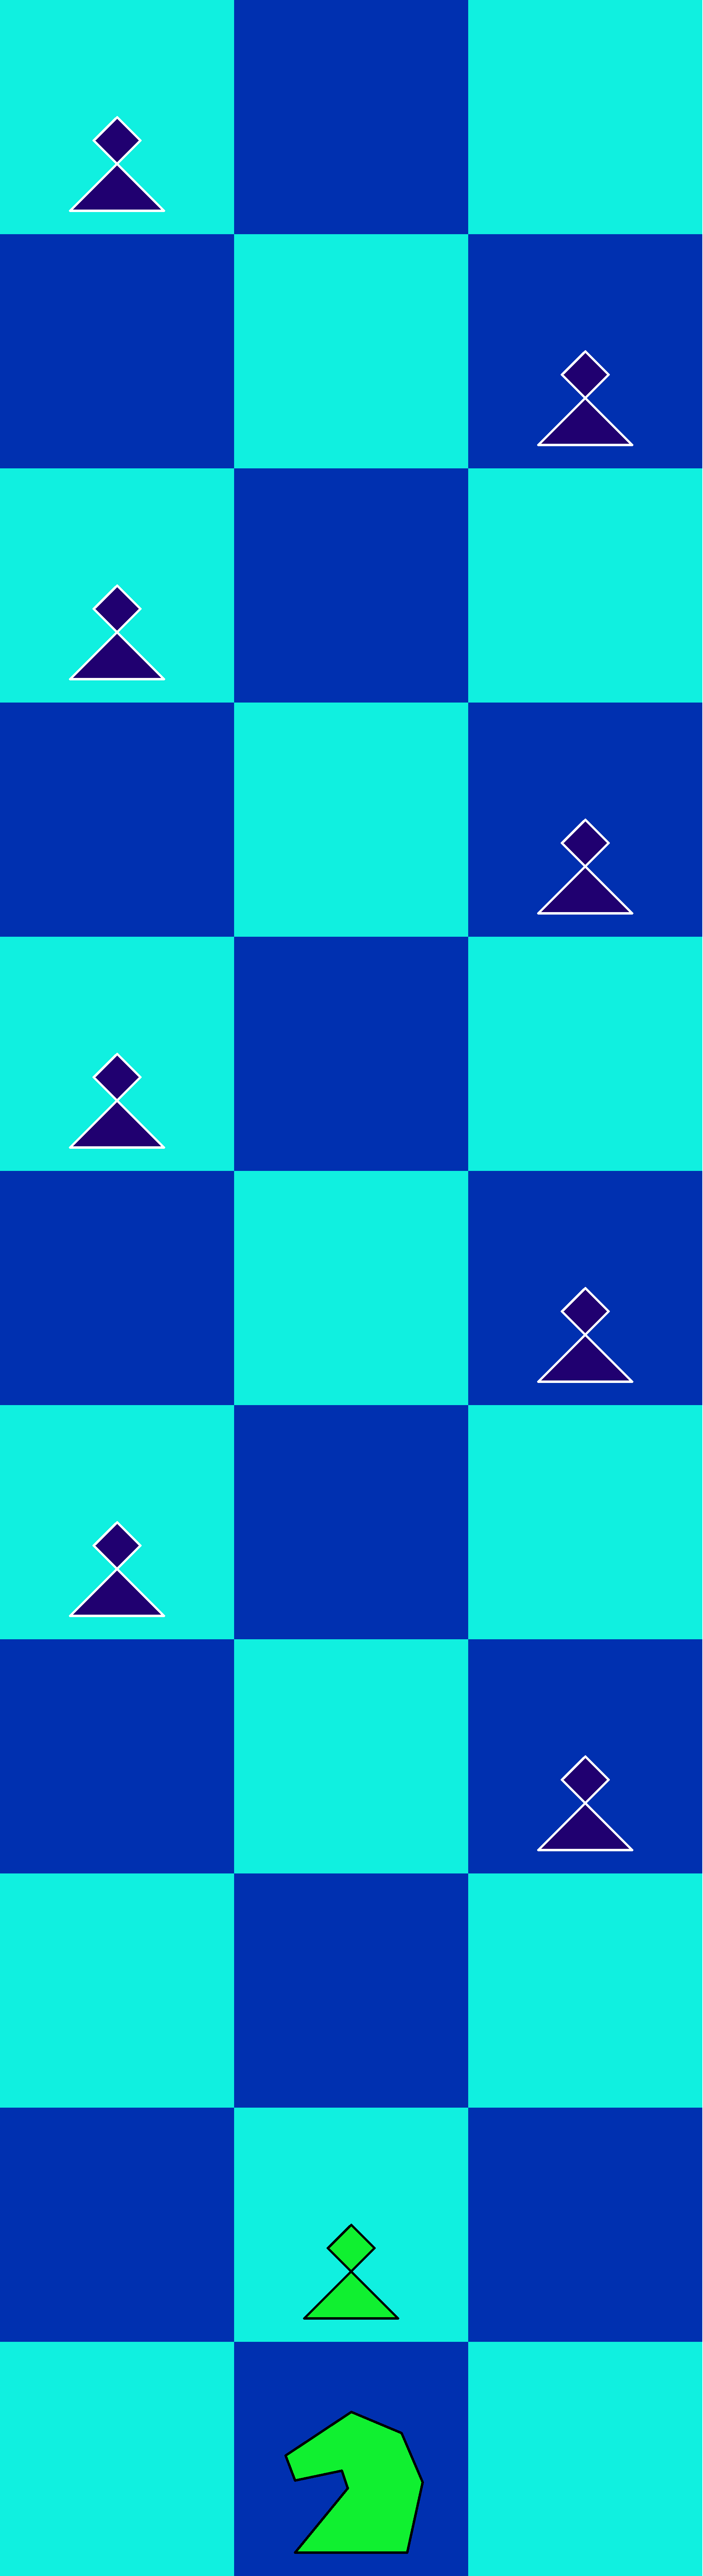
\includegraphics[width=1.0\textwidth, keepaspectratio=true]{en_passants/16_tamoanchan_revisited_en_passant.png}
\caption{En passant}
\label{fig:16_tamoanchan_revisited_en_passant}
\end{figure}

Rush and en passant are identical to those in \hyperref[fig:14_hemera_s_dawn_en_passant]{Hemera's Dawn variant}.
Own Pawns can be rushed for up to 9 fields in this variant.

\clearpage % ..........................................................

\section*{Promotion}
\addcontentsline{toc}{section}{Promotion}
\label{sec:Tamoanchan Revisited/Promotion}

Promotion is non enforced, delayed variety, i.e. it's the same as in
\hyperref[sec:Age of Aquarius/Promotion]{previous chess variant}, Age of Aquarius.

Promotion in this variant is polygamous, more than one Queen in the same color
can be present on chessboard at any given time.

% \clearpage % ..........................................................

\section*{Castling}
\addcontentsline{toc}{section}{Castling}
\label{sec:Tamoanchan Revisited/Castling}

Castling is
\hyperref[sec:Nineteen/Castling]{the same as in Nineteen variant},
only difference is that King can move
between 2 and 8 fields across. All other constraints from Nineteen variant still
applies.

\noindent
\begin{figure}[!h]
\includegraphics[width=1.0\textwidth, keepaspectratio=true]{castlings/16_tr/tamoanchan_revisited_castling.png}
\caption{Castling}
\label{fig:tamoanchan_revisited_castling}
\end{figure}

In example above, all valid King's castling moves are numbered.

\noindent
\begin{figure}[!h]
\includegraphics[width=1.0\textwidth, keepaspectratio=true]{castlings/16_tr/tamoanchan_revisited_castling_left_03.png}
\caption{Castling short left}
\label{fig:tamoanchan_revisited_castling_left_03}
\end{figure}

In this example King was castling short to the left. Initial King's position is
marked with "K". After castling is finished, left Rook ends up at field immediately
right to the King.

\clearpage % ..........................................................

\section*{Initial setup}
\addcontentsline{toc}{section}{Initial setup}
\label{sec:Tamoanchan Revisited/Initial setup}

Compared to initial setup of Hemera's Dawn, Serpent is put onto inner field next
to Bishop symmetrically, on both sides of chessboard, some figures are also
repositioned. This can be seen in the image below:

\noindent
\begin{figure}[h]
\includegraphics[width=1.0\textwidth, keepaspectratio=true]{boards/16_tamoanchan_revisited.png}
\caption{Tamoanchan Revisited board}
\label{fig:16_tamoanchan_revisited}
\end{figure}

\clearpage % ..........................................................
% ======================================== Tamoanchan Revisited chapter
